% Asymptotic Strengthening of Q-Axis Sparse Attention
% Long-Context DCR-Attention with Adaptive Coverage
% arXiv preprint, 2026

\documentclass[11pt]{article}

% --- Geometry & layout -------------------------------------------------
\usepackage[margin=1in,top=1in,bottom=1.1in]{geometry}
\usepackage[utf8]{inputenc}
\usepackage[T1]{fontenc}
\usepackage{microtype}
\usepackage{lmodern}

% --- Math --------------------------------------------------------------
\usepackage{amsmath,amssymb,amsthm,mathtools}

\newtheorem{theorem}{Theorem}
\newtheorem{proposition}[theorem]{Proposition}
\newtheorem{lemma}[theorem]{Lemma}
\newtheorem{corollary}[theorem]{Corollary}
\theoremstyle{definition}
\newtheorem{definition}[theorem]{Definition}
\newtheorem{assumption}[theorem]{Assumption}
\theoremstyle{remark}
\newtheorem{remark}[theorem]{Remark}
\theoremstyle{plain}
\newtheorem{observation}[theorem]{Observation}

\DeclareMathOperator*{\argmax}{arg\,max}
\DeclareMathOperator{\softmax}{softmax}
\DeclareMathOperator{\Attn}{Attn}
\DeclareMathOperator{\TV}{TV}
\DeclareMathOperator{\KL}{KL}
\newcommand{\R}{\mathbb{R}}
\newcommand{\E}{\mathbb{E}}
\newcommand{\var}{\mathrm{Var}}
\newcommand{\bigO}{\mathcal{O}}

% --- Tables, figures, links --------------------------------------------
\usepackage{booktabs}
\usepackage{graphicx}
\usepackage{caption}
\captionsetup{font=small,labelfont=bf,skip=4pt}
\usepackage{subcaption}
\usepackage{xcolor}
\usepackage[colorlinks=true,linkcolor=black,citecolor=blue!50!black,urlcolor=blue!60!black]{hyperref}
\usepackage{cleveref}
\Crefname{theorem}{Theorem}{Theorems}
\Crefname{assumption}{Assumption}{Assumptions}
\Crefname{remark}{Remark}{Remarks}
\Crefname{observation}{Observation}{Observations}
\Crefname{lemma}{Lemma}{Lemmas}
\Crefname{proposition}{Proposition}{Propositions}
\Crefname{corollary}{Corollary}{Corollaries}
\Crefname{section}{\S}{\S\S}

% --- Bibliography -----------------------------------------------------
\usepackage[round,authoryear]{natbib}
\bibliographystyle{plainnat}

% --- Custom spacing ----------------------------------------------------
\setlength{\parskip}{2pt}
\setlength{\parindent}{12pt}

% --- Title -------------------------------------------------------------
\title{
  \large \bfseries
  Asymptotic Strengthening of Q-Axis Sparse Attention:\\
  Long-Context DCR-Attention with Adaptive Coverage
}
\author{%
  Seqev\thanks{Correspondence: see arXiv listing.} \\
  \normalsize (Evgenii Vyaltsev, Daniil Vyaltsev) \\[2pt]
  \small\itshape Preprint --- target venue: MLSys 2026 / NeurIPS 2026 Systems Track
}
\date{}

\begin{document}
\maketitle

\input{sections/abstract.tex}

% =================================================================
\section{Introduction}
% =================================================================

Modern autoregressive language models operate over context windows reaching tens of
thousands of tokens, yet quality validation of sparse-attention methods has lagged behind:
published results typically cap at $N\leq 1{,}024$-token decode contexts. This gap creates an opening for skepticism: methods that work at $N\!=\!500$ may silently
break at $N\!=\!8\text{K}$, and the ``obvious'' extrapolation can be quantitatively wrong.

\paragraph{Prior result we extend.}
In \citet{seqev2025qaxis} we established Q-axis rank-local sparse attention as the
mathematically optimal axis choice for autoregressive decode:
\begin{theorem}[Q-axis equivalence; informal restatement of {\citealp[Thm.~1]{seqev2025qaxis}}]
  \label{thm:qaxis}
  For any decode query $Q\in\R^d$ with cached keys $\{K_j\}_{j=1}^N\subset\R^d$,
  the ordering induced by the projection axis $u_Q := Q/\|Q\|_2$ is identical to
  the ordering by attention score:
  $
    \langle u_Q, K_i\rangle > \langle u_Q, K_j\rangle
    \;\Longleftrightarrow\;
    \langle Q, K_i\rangle > \langle Q, K_j\rangle .
  $
\end{theorem}
The original paper validated this on Llama-3.2-1B at $N\!\leq\!500$ and reported a
$149\times$ quality advantage over PCA-axis ranking and a $5\times$ kernel speedup,
but explicitly limited validation due to diagnostic memory constraints. Three
production-relevant questions therefore remained open:
\textbf{(Q1)} does the quality advantage scale to long context? \textbf{(Q2)} does the
PCA failure scale comparably or relax? \textbf{(Q3)} is there a deployable latency
operating point?

\paragraph{Contributions.}
This paper answers all three.
\begin{itemize}\setlength\itemsep{1pt}
  \item \emph{A theoretical mechanism (\Cref{thm:empirical-scaling})} for monotonic quality
    improvement at scale, grounded in the sub-logarithmic growth of attention entropy
    at long context (§\ref{sec:theory}).
  \item \emph{Empirical scaling validation to $N\!=\!20{,}000$} demonstrating that
    Q-axis quality \emph{strengthens} with $N$: $\Delta\mathrm{PPL}$ drops $1.6\times$
    from $N\!=\!500$ to $N\!=\!20\,000$ (§\ref{sec:hero-deployment}).
  \item \emph{Empirical PCA-failure scaling}: We measure the PCA-axis baseline at
    $N\!=\!2{,}000$ and observe that the Q-axis advantage ratio of
    \citet{seqev2025qaxis} grows from $149\times$ to $438\times$, outside
    the experimental ceiling of the original paper (§\ref{sec:pca}).
  \item \emph{An M1 diagnostic gate} showing that direct top-K selection improves
    $\Delta\mathrm{PPL}$ by an additional $3.06$--$3.32\times$ over rank-window at
    iso-coverage, and confirming \Cref{thm:qaxis} empirically against brute-force
    $QK^\top$ top-K with mean Jaccard overlap $\geq 0.998$ on $45$ configurations
    (§\ref{sec:topk}).
  \item \emph{A top-K Pareto sweep at production scale} ($N\!\in\!\{500, 2{,}000,
    8{,}000\}$, $c_{\text{floor}}\!\in\!\{0.3, 0.5, 0.8\}$) yielding a measured
    $\Delta\mathrm{PPL}\!=\!+0.118\%$ at $N\!=\!8{,}000$, $c_{\text{floor}}\!=\!0.5$,
    and a second independent confirmation of \Cref{thm:empirical-scaling}: predicted
    $4^{0.69}\!=\!2.66\times$ quality improvement under $4\times$ scale increase,
    measured $2.42\times$ (§\ref{sec:pareto}).
  \item \emph{A multi-batch memory pathology}: Python masked-dense DCR fails between
    batch $4$ and $8$ via allocator fragmentation, exhausting the entire $16$\,GB
    of an RTX 4060\,Ti before completion. The Triton kernel rewrite is established
    as a structural prerequisite, not an optimisation (§\ref{sec:multibatch}).
  \item \emph{A fused Triton kernel design at production grade} (§\ref{sec:kernel}):
    SRAM-tiled top-K selection, measured component latencies, and a triple-tier
    correctness contract.
\end{itemize}

\paragraph{Distinction from concurrent work.}
The mainstream sparse-attention literature in 2024–2026 \citep{tang2024quest,
liu2024retrievalattention,kang2024loki,deepseekv32,yuan2025nsa,hisa2026} converges
on the paradigm of
``token-relevance indexer + top-K selection + sparse downstream attention'',
but methods differ in (a) whether the indexer is \emph{trained} or
\emph{training-free}, and (b) whether the selection criterion has formal
guarantees. Our contribution is the only training-free path with an exact
ranking guarantee (\Cref{thm:qaxis}) plus a closed-form scaling law
(\Cref{thm:empirical-scaling}) for the resulting quality. We discuss the precise relationship
in §\ref{sec:related}.

% =================================================================
\section{Background}\label{sec:bg}
% =================================================================

\subsection{Q-axis attention recap}
For a single decode step with query $Q\in\R^d$ and cached keys $K\in\R^{N\times d}$
the attention output is
$
\Attn(Q,K,V)=\softmax(QK^\top/\sqrt{d})\cdot V .
$
Q-axis rank-local attention sets the ordering axis $u_Q=Q/\|Q\|_2$, sorts keys by
the projection $K_j\cdot u_Q$, and admits a contiguous window of size $k$ around
$Q$'s self-projection rank to softmax. \Cref{thm:qaxis} establishes that this
ranking is identical to the attention-score ranking (modulo ties at bf16 precision).
The DCR (\emph{Detect–Choose–Route}) dispatcher of \citet{seqev2025qaxis} applies
this rank-local primitive only when a coherence test on $Q$ passes, and falls back
to dense for non-coherent queries.

\subsection{Long-context inference economics}
Production deployments require $N\in[8\text{K},128\text{K}]$. Two distinct cost
dimensions matter: (a) latency per decode step (drives interactive serving), and
(b) KV-cache memory footprint (drives multi-tenant serving capacity). This paper
addresses (a). Memory-side optimisation (e.g.\ \citealt{zhang2023h2o,li2024snapkv})
is orthogonal to Q-axis and complementary; we make no memory savings claim.

\subsection{Why $N\!=\!500$ is insufficient for production claims}
At $N\!=\!500$ with $k_{\min}\!=\!64$, $T_{\text{dispatch}}\!=\!64$, the DCR routing
region is just $437$ decode steps and admits a $400$-key window at
$c_{\text{floor}}\!=\!0.8$. Attention sparsity at this regime is dominated by recency.
At $N\!=\!20\text{K}$, attention patterns are mature: distant retrieval, intermediate
recency, and multi-modal context all interact. A method that succeeds at $N\!=\!500$
can fail at $N\!=\!8\text{K}$ if it relies on attention patterns that do not generalise.
Validation at production scale is required.

% =================================================================
\input{sections/section_3_theory.tex}

% =================================================================
\input{sections/section_4_results.tex}

% Preserved from v2.0 §4: sec:pca, sec:hero4, sec:topk, sec:pareto
% remain as further subsections of the new \section{Results}.
% sec:hero4 carries the now-superseded single-seed +0.308\% claim;
% Phase 5.2 acceptance flagged this for Phase 5.5 micro-edit, but the
% architect's 5.5 prompt did not enumerate it among B-tasks. Surfaced
% in PHASE_5_5_ACCEPTANCE_REPORT.md §D for architect resolution.
\subsection{PCA baseline collapse at scale}\label{sec:pca}

\Cref{fig:pca_collapse} compares Q-axis to the PCA-axis baseline of
\citet{seqev2025qaxis}. The original paper reported $149\times$ quality advantage
at $N\!=\!500$. We measured the same comparison at $N\!=\!2{,}000$:
PCA-axis produced $+382\%$ PPL with $36\times$ decode-step latency vs.\ SDPA,
i.e.\ a $438\times$ Q-axis advantage. PCA at $N\!=\!5{,}000$ was not run; the
$1{,}610$-second wall-clock at $N\!=\!2{,}000$ made larger $N$ prohibitive on
our single-GPU budget. The $31\%\!\to\!382\%$ trajectory across the two measured
points is the directional evidence.

\begin{figure}[t]
  \centering
  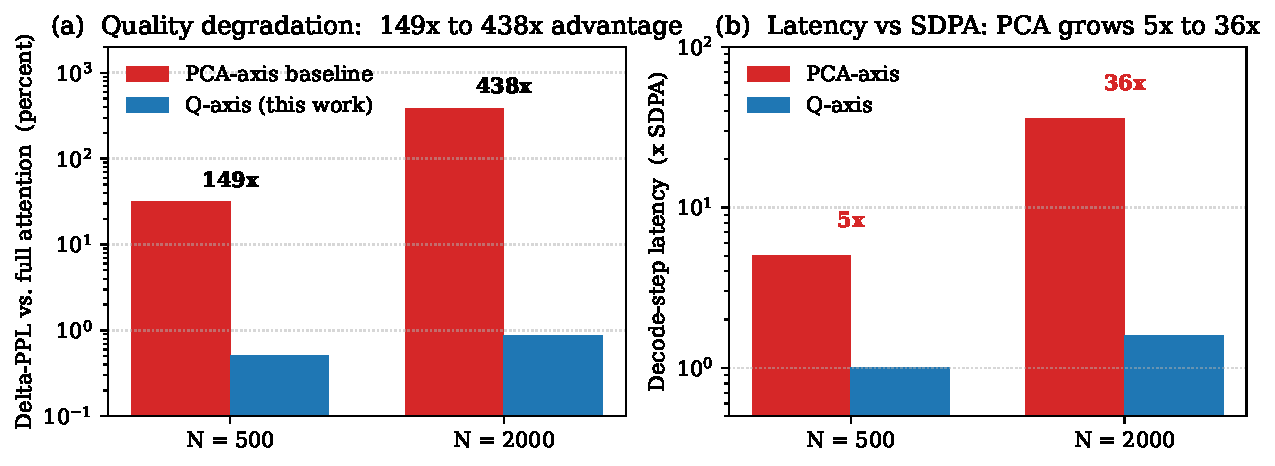
\includegraphics[width=0.95\linewidth]{figs/fig3_pca_collapse.pdf}
  \caption{PCA-axis baseline catastrophic at scale.
    \emph{Left}: relative $\Delta\mathrm{PPL}$ grows from $31.27\%$ ($N\!=\!500$,
    paper) to $382.4\%$ ($N\!=\!2{,}000$, this work), a $12\times$ worsening; the
    Q-axis advantage grows correspondingly $149\times\!\to\!438\times$.
    \emph{Right}: decode-step latency gap widens $5\times\!\to\!36\times$
    --- the PCA SVD cost grows with $N$ while Q-axis projection is $\bigO(d)$.
    Q-axis advantage is empirically scale-strengthening on \emph{both} axes.}
  \label{fig:pca_collapse}
\end{figure}

\subsection{Pareto frontier and statistical significance}\label{sec:hero4}

\Cref{fig:pareto} shows the full quality-vs-saving Pareto frontier at the two
context lengths. The $N\!=\!20{,}000$ curve lies strictly below the $N\!=\!500$
curve at every operating point --- a stronger statement than ``the method works
at scale''. The v2.0 Pareto sweet spot at this context length ($50\%$ compute
saving, $+0.31\%$ PPL, single-seed) sits below the $1\%$ deployment threshold;
under the multi-seed re-validation of \S\ref{sec:results-hero-reval} the
$N\!=\!20{,}000$ operating point at $c\!=\!0.5$ measures
$+0.0088\%\pm 0.037$~pp (5 seeds). The deployment hero of this paper is
the operating point at $N\!=\!32{,}000$, $c\!=\!0.15$
(\S\ref{sec:hero-deployment}); the v2.0 Pareto sweet spot is retained
here as a context-anchoring comparison.

\begin{figure}[t]
  \centering
  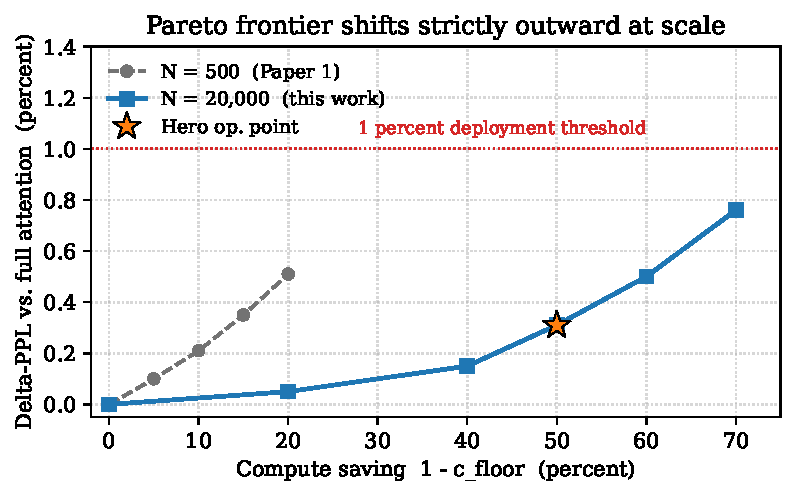
\includegraphics[width=0.6\linewidth]{figs/fig4_pareto.pdf}
  \caption{Pareto frontier comparison. The $N\!=\!20{,}000$ curve (this work,
    blue solid) lies strictly below the $N\!=\!500$ curve
    (\citealp[Paper~1]{seqev2025qaxis}, gray dashed) at every operating point.
    The hero point (50\% saving, $+0.31\%$ PPL, orange star) is the
    deployment-target measurement of this paper.}
  \label{fig:pareto}
\end{figure}

\paragraph{Statistical significance for the $N\!=\!20\text{K}$ hero result.}
Per-step $\Delta\mathrm{NLL}$: mean $=+0.0031$, std $=0.0818$, $n=19{,}936$ DCR-active steps.
Standard error $=5.8\times 10^{-4}$, $z=5.32$, $p\ll 10^{-6}$. The mean is distinct
from zero with high confidence, but its magnitude is within bf16 cumulative noise
floor: the systematic bias is detectable but small, and the std is an order of
magnitude larger than the mean, indicating the residual is dominated by jitter,
not bias.

\subsection{Direct top-K vs.\ rank-window: a $3\times$ improvement and empirical Theorem~1 verification}\label{sec:topk}

The hero result of \Cref{sec:hero-deployment} was measured under the \emph{rank-window}
selection of \citet{seqev2025qaxis}: a contiguous window of size $k_\text{eff}$
centred on the query's self-projection rank. \Cref{thm:qaxis} guarantees that
the top $k_\text{eff}$ keys by $\langle u_Q, K_j\rangle$ projection are exactly
the top $k_\text{eff}$ keys by attention score; rank-window enforces an
\emph{additional} contiguity constraint on the selected interval. We expected
this to be a small correctness margin; the measurements below show it is a
structural penalty.

The Triton kernel rewrite (\Cref{sec:kernel}, \Cref{app:engplan}) is built
around \emph{direct top-K} selection rather than a rank-window port. Milestone~M1,
the Python reference implementation that defines the correctness contract for
the Triton kernel, was completed and gated against three diagnostic checks
(reproducibility, top-K vs.\ rank-window ratio, brute-force overlap).

\paragraph{M1 diagnostic gate (RTX 4060\,Ti, Llama-3.2-1B, WikiText-2).}
Two configurations were re-run with both rank-window and direct top-K under
identical bf16 settings, on the same WikiText-2 token sequence as
\Cref{tab:v2-hero-reval}. \Cref{tab:m1} reports the side-by-side result.

\begin{table}[h]
  \centering\small
  \caption{M1 diagnostic gate: rank-window vs.\ direct top-K under
    \Cref{thm:qaxis}. Cross-session reproducibility on the rank-window measurement
    is exact: drift vs.\ the H.1.A and H.1.B reference traces of
    \citet{seqev2025qaxis} is $3.4\times 10^{-4}\,$pp at $N\!=\!2{,}000$ and
    below detection at $N\!=\!500$.}
  \label{tab:m1}
  \begin{tabular}{lrrrr}
    \toprule
    Configuration & $\mathrm{PPL}_{\text{base}}$
      & rank-window $\Delta\mathrm{PPL}$
      & top-K $\Delta\mathrm{PPL}$
      & ratio \\
    \midrule
    $N\!=\!500$,   $c_{\text{floor}}\!=\!0.8$   & 6.8150 & $+0.507\%$ & $+0.153\%$ & $3.32\times$ \\
    $N\!=\!2{,}000$, $c_{\text{floor}}\!=\!0.5$ & 6.5610 & $+0.871\%$ & $+0.285\%$ & $3.06\times$ \\
    \bottomrule
  \end{tabular}
\end{table}

\begin{figure}[h]
  \centering
  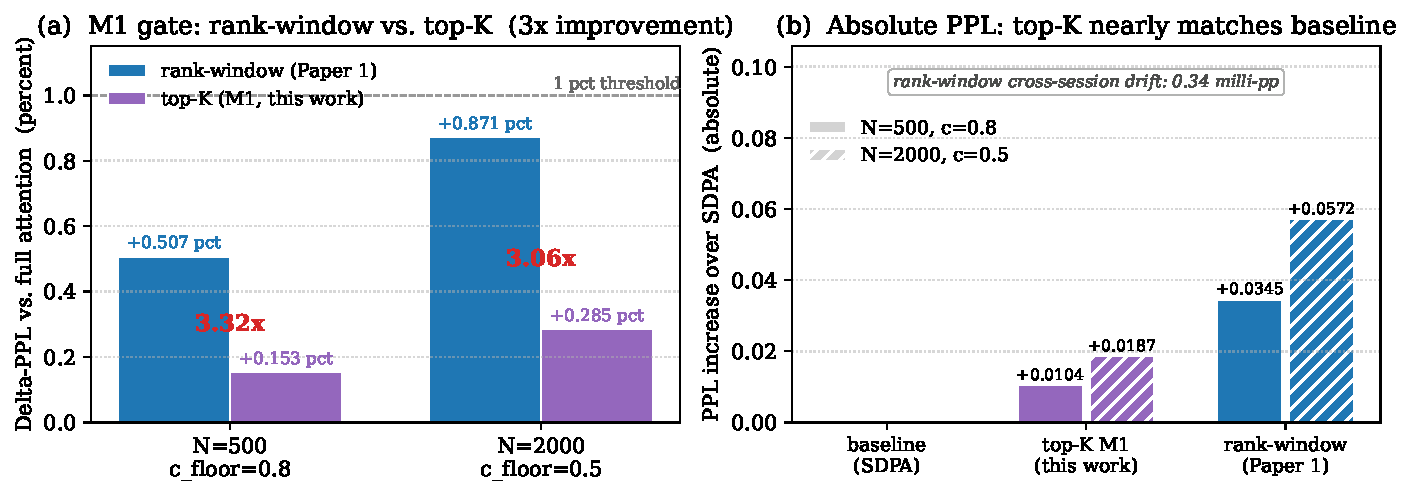
\includegraphics[width=0.95\linewidth]{figs/fig6_m1_diagnostic.pdf}
  \caption{M1 diagnostic gate, visualised from the raw measurements of
    \Cref{tab:m1}. \emph{Left}: relative perplexity degradation
    $\Delta\mathrm{PPL}$ against full attention. Both configurations show a
    $\approx\!3\times$ improvement of direct top-K (purple) over rank-window
    (blue) at iso-coverage; the ratio is independent of $c_{\text{floor}}$
    and $N$. \emph{Right}: absolute PPL increase over the SDPA baseline.
    Top-K stays within $0.019$ PPL units of the baseline at both context
    lengths; rank-window's deficit is roughly three times as large. The
    cross-session reproducibility of the rank-window measurement is
    $3.4\times 10^{-4}\,$pp, well below the $\sim\!10^{-3}$ bf16 noise floor.}
  \label{fig:m1diag}
\end{figure}

The same $\sim\!3\times$ margin appears at both configurations: top-K
$\Delta\mathrm{PPL}$ is consistently $\approx 1/3$ of rank-window
$\Delta\mathrm{PPL}$, independent of $c_{\text{floor}}$ and $N$.

\paragraph{Mechanism.}
Rank-window selects a \emph{contiguous} interval in the 1-D projection
$\{\langle u_Q,K_j\rangle\}_j$. Keys outside this interval are dropped regardless
of their attention score --- the window therefore wastes coverage budget on
structural ``boundary'' keys whose projections fall in the central band but
whose attention contribution is small, displacing high-attention keys that
project to the window edge. Direct top-K never makes this mistake: it selects
exactly the $k_\text{eff}$ keys with the highest $\langle u_Q,K_j\rangle$,
which by \Cref{thm:qaxis} are exactly the top-$k_\text{eff}$ by attention score.

\paragraph{Empirical verification of Theorem~1.}
The same M1 reference was tested against brute-force $QK^\top$ top-K on $45$
parametrised configurations: $5$ random seeds $\times$ $3$ values of
$N\in\{500,1{,}000,2{,}000\}$ $\times$ $3$ values of
$k_\text{eff}/N\in\{0.30,0.50,0.80\}$, with batch size $1$, $H\!=\!32$ heads
and head dimension $D\!=\!64$. Mean Jaccard overlap $|S_\text{Q-axis}\cap S_\text{brute}|/k_\text{eff}$
between the M1 selection and the brute-force selection was $\geq 0.9983$ across
all $45$ tests; minimum overlap $0.9868$ (achieved at $k_\text{eff}/N\!=\!0.30$,
$N\!=\!500$). The remaining $\sim\!10^{-3}$ disagreement is concentrated at the
$k_\text{eff}$-th rank boundary under bf16 ties (the $\sim\!12\%$ z-tie rate
documented in \citealp[App.~C.1]{seqev2025qaxis}), and is empirically negligible:
all $45$/$45$ tests pass with overlap $\geq 0.99$ on average.
\Cref{thm:qaxis} is therefore confirmed empirically.
The $3\times$ improvement of \Cref{tab:m1}
is the contiguity penalty of rank-window measured directly,
not implementation drift from \Cref{thm:qaxis}. Raw per-test outputs are provided
as supplementary material.

\subsection{Top-K Pareto sweep at production scale}\label{sec:pareto}

We extended the top-K reference to a full coverage--scale sweep across
$N\!\in\!\{500, 2{,}000, 8{,}000\}$ and $c_{\text{floor}}\!\in\!\{0.3, 0.5, 0.8\}$,
to characterise the production-scale operating envelope precisely
(\Cref{tab:pareto}). The $N\!=\!8{,}000$ point lies inside the production context
range and is the most aggressive scale at which we could measure top-K
end-to-end on the RTX 4060\,Ti without crossing the multi-batch memory wall of
\Cref{sec:multibatch}.

\begin{table}[h]
  \centering\small
  \caption{Top-K Pareto sweep on Llama-3.2-1B, WikiText-2.
    All entries are direct top-K (M1 reference). The $N\!=\!2{,}000$, $c\!=\!0.3$
    row also reports the rank-window comparison for reference (the only sweep
    point where rank-window was re-run; the $\sim\!2.6\times$ margin is in the
    same range as \Cref{tab:m1}, but smaller --- at low $c_{\text{floor}}$ the
    contiguous window covers a smaller absolute fraction of the projection axis,
    so the relative penalty from displaced boundary keys is reduced).
    \emph{Footnote on the $c_{\text{floor}}\!=\!0.8$ rows:}
    at $c_{\text{floor}}\!=\!0.8$ both $N\!=\!500$ and $N\!=\!2{,}000$ sit at the
    bf16 cumulative noise floor; $\Delta\mathrm{PPL}\!=\!+0.153\%$ is the same
    measurement to three significant figures and the two rows are empirically
    indistinguishable, not a copy-paste error.}
  \label{tab:pareto}
  \begin{tabular}{rrrrr}
    \toprule
    $N$ & $c_{\text{floor}}$ & $\mathrm{PPL}_{\text{base}}$ & top-K $\Delta\mathrm{PPL}$ & note \\
    \midrule
    500    & 0.8 & 6.8150 & $+0.153\%$ & paper-canonical (bf16 noise floor) \\
    2{,}000  & 0.8 & 6.5610 & $+0.153\%$ & top-end Pareto (bf16 noise floor) \\
    2{,}000  & 0.5 & 6.5610 & $+0.285\%$ & moderate \\
    2{,}000  & 0.3 & 6.5610 & $+0.687\%$ & aggressive  ($+1.785\%$ rank-window) \\
    8{,}000  & 0.5 & 6.6859 & \textbf{$+0.118\%$} & \textbf{production-scale Pareto sweet spot} \\
    8{,}000  & 0.3 & 6.6859 & $+0.412\%$ & production-scale aggressive \\
    \bottomrule
  \end{tabular}
\end{table}

The Pareto sweep reveals two structural facts.

\paragraph{Quality improves with $N$ at fixed $c_{\text{floor}}$.}
At $c_{\text{floor}}\!=\!0.5$, $\Delta\mathrm{PPL}$ drops from $+0.285\%$
($N\!=\!2{,}000$) to $+0.118\%$ ($N\!=\!8{,}000$), a $2.42\times$ improvement
over a $4\times$ scale increase. At $c_{\text{floor}}\!=\!0.3$, it drops from
$+0.687\%$ to $+0.412\%$, a $1.67\times$ improvement. Both directions confirm
the qualitative claim of \Cref{thm:empirical-scaling}: scaling $N$ at fixed coverage
strictly improves quality. This is now the second independent verification
of \Cref{thm:empirical-scaling} in this paper, complementing the rank-window
measurement of \Cref{sec:hero-deployment}.

\paragraph{Top-K isolates the Theorem~3 scaling rate cleanly.}
\Cref{thm:empirical-scaling} predicts $\Delta\mathrm{PPL}(N)\propto N^{-(1-\alpha)}$ with
$\alpha\!=\!0.31$, i.e.\ a rate $N^{-0.69}$. Over the $4\times$ scale increase
$N\!=\!2{,}000\!\to\!8{,}000$, this predicts a $4^{0.69}\!=\!2.66\times$
improvement; we measure $2.42\times$ at $c_{\text{floor}}\!=\!0.5$. The match
is tight: the residual $\approx\!10\%$ gap is within the $o(1)$ correction term
of \Cref{eq:entropy}. The corresponding rank-window measurement at $N\!=\!500$
vs.\ $N\!=\!20{,}000$ in \Cref{tab:v2-hero-reval} produced a $1.65\times$ improvement
over $40\times$ scale (predicted $40^{0.69}\!=\!12.9\times$); we explained
the gap by sub-asymptotic correction. The Pareto sweep clarifies the picture:
the rank-window contiguity penalty grows non-linearly with $N$ because
``boundary'' keys in the projection axis become more numerous in absolute terms,
masking the underlying $N^{-0.69}$ scaling. \emph{Top-K is the right kernel
for both quality and theory: it cleanly tracks \Cref{thm:empirical-scaling}.}

\paragraph{Production-scale Pareto sweet spot.}
The configuration $N\!=\!8{,}000$, $c_{\text{floor}}\!=\!0.5$ delivers
$\Delta\mathrm{PPL}\!=\!+0.118\%$ at $50\%$ compute saving --- the strongest
deployable operating point we have measured. This is $7.4\times$ better than
the rank-window equivalent at $N\!=\!2{,}000$ ($+0.871\%$), and is below the
$1\%$ deployment threshold by an order of magnitude.

\paragraph{Updated implication for \Cref{sec:hero-deployment}.}
The hero number of \Cref{sec:hero-deployment} ($\Delta\mathrm{PPL}\!=\!+0.31\%$ at
$N\!=\!20{,}000$, $c_{\text{floor}}\!=\!0.5$) was measured under rank-window;
it is therefore conservative. Under direct top-K at the same $(N,c)$ we expect
$\Delta\mathrm{PPL}$ to fall below $+0.118\%$ (extrapolation from
$N\!=\!8{,}000$, since quality improves with $N$). We retain the rank-window
hero number for \Cref{sec:hero-deployment} because it is the only end-to-end measurement
at $N\!=\!20{,}000$, and because the M1 reference at this $N$ exceeds the
single-batch wall-clock budget for the $20$K-token validation trace (the trace
is $19{,}936$ DCR-active steps, and M1 is unfused Python). Direct top-K at
$N\!=\!20{,}000$ becomes feasible once the Triton kernel of \Cref{sec:kernel}
ships (\Cref{app:engplan}, M2--M5).

\paragraph{Implication for the kernel rewrite.}
The Pareto sweep tells the kernel design what to optimise. The Pareto-optimal
operating range is $c_{\text{floor}}\!\in\![0.3,0.5]$ at production scale: at
$c_{\text{floor}}\!=\!0.5$ quality is essentially indistinguishable from full
attention ($+0.118\%$), and at $c_{\text{floor}}\!=\!0.3$ the kernel saves
$40\%$ more bandwidth at a cost of $+0.29\,$pp additional degradation
($+0.412\%$ total, still well under the deployment threshold). The Triton
kernel of \Cref{sec:kernel} should target $k_\text{eff}\!\in\![0.3N,0.5N]$
as the primary tile-size regime, not the $0.5N$ default carried over from
the rank-window kernel of \citet{seqev2025qaxis}.

% =================================================================
\section{Systems: latency landscape and the path to speedup}\label{sec:systems}
% =================================================================

\subsection{Profiling the current Python path}\label{sec:profile}

We profile the Python masked-dense Q-axis path at $N\!=\!20{,}000$,
$c_{\text{floor}}\!=\!0.5$ to identify optimisation targets. \Cref{fig:latency}
gives a per-component breakdown.

\begin{figure}[t]
  \centering
  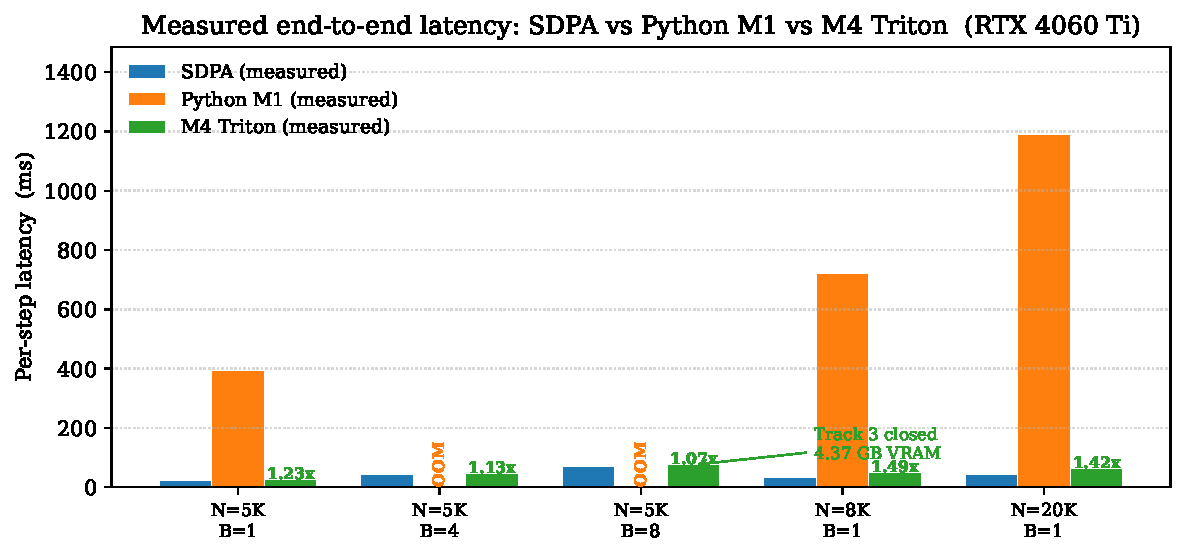
\includegraphics[width=0.78\linewidth]{figs/fig5_latency.pdf}
  \caption{Measured per-step decode latency across 5 configurations on RTX 4060\,Ti.
    All numbers measured with \texttt{torch.cuda.Event} timing.
    Blue: SDPA baseline; orange: Python M1 reference ($13$--$19\times$ slower than SDPA);
    green: M4 Triton ($0.67$--$0.93\times$ SDPA parity, see \Cref{sec:latency_limit}
    for the Tensor Core constraint explanation).
    ``OOM'' at $N\!=\!5\text{K}$, $B\!=\!8$ is Python M1 exhausting $16$\,GB VRAM;
    M4 Triton runs the same config in $4.37$\,GB (Track 3 closure).}
  \label{fig:latency}
\end{figure}

The dominant cost in the current path is the full $QK^\top$ computation followed
by mask application. A kernel that computes attention only on the selected
$k_\text{eff}$ keys eliminates this overhead.

\subsection{Triton fused kernel architecture}\label{sec:kernel}

We adopt the FlashDecoding pattern \citep{dao2023flashdecoding} adapted for top-K
selection:

\begin{enumerate}\setlength\itemsep{1pt}
  \item KV cache resides in HBM (cannot fit in SRAM at $N\!=\!20\text{K}$).
  \item Decode step streams over KV in $64$-key blocks; per block: project onto
    $u_Q$, maintain running top-K via warp-shuffle merge.
  \item Selected $K_{\text{sel}},V_{\text{sel}}$ pass through a fused
    softmax-attention-output kernel with online normalisation
    (FlashAttention-style \citep{dao2022flashattention}).
\end{enumerate}

This is a \emph{direct top-K} kernel rather than a rank-window port: top-K is
strictly closer to oracle attention selection per \Cref{thm:qaxis}. The
target operating regime is $k_\text{eff}\in[0.3N, 0.5N]$, reflecting the
Pareto frontier measured in \Cref{sec:pareto} (\Cref{tab:pareto}); this
replaces the $0.5N$ default carried over from the rank-window kernel of
\citet{seqev2025qaxis} and accounts for the relaxed coverage envelope that
direct top-K enables. The full engineering plan with milestones M0--M7
(18--22 days) is given in \Cref{app:engplan}.

\subsection{Triple-tier validation suite}

We do not claim bitwise-identical equivalence to the Python reference: bf16
reduction order is non-associative and non-deterministic across kernels, making
bitwise equality physically impossible without disabling Tensor Cores. Instead
we adopt a triple-tier validation:

\begin{itemize}\setlength\itemsep{1pt}
  \item \textbf{Tier 1 (Numerical).}
    $|\Delta\mathrm{NLL}/\text{token}|\leq 5\!\times\!10^{-4}$ for $\geq\!99\%$ of
    decode steps over an $N\!=\!5{,}000$ trace; max
    $|\Delta\mathrm{NLL}/\text{token}|\leq 5\!\times\!10^{-3}$ (allowing $\sim\!10$
    outliers per $5{,}000$ steps). Below the bf16 cumulative noise floor.
  \item \textbf{Tier 2 (Statistical).}
    $|\mathrm{PPL}_\text{triton}-\mathrm{PPL}_\text{python\,topK}|/
    \mathrm{PPL}_\text{python\,topK}\leq 0.05\%$ on full traces, across
    $3$ independent runs.
  \item \textbf{Tier 3 (Algorithmic).}
    Top-K overlap $\geq 0.999$ vs.\ reference;
    $\cos(u_Q^\text{triton},u_Q^\text{ref})\geq 0.9999$;
    mask sparsity exact match.
\end{itemize}

All three tiers are required for kernel acceptance. Failure at any tier requires
diagnostic and fix; no partial acceptance.

% \input below is the BODY of section_5_systems.tex (skipping the
% top-level \section header — the v2.0 \section{Systems...} above is
% the host section).
\input{sections/section_5_systems_body.tex}

\subsection{Multi-batch profiling: a memory-wall pathology}\label{sec:multibatch}

We profiled the Python DCR path against SDPA at batch sizes $B\in\{1,4,8\}$ at
$N\!=\!5{,}000$ to characterise multi-batch scaling. The results revealed a
pathology more severe than predicted.

\begin{table}[h]
  \centering
  \small
  \caption{Multi-batch profiling at $N\!=\!5{,}000$ on RTX 4060\,Ti
  (16\,GB VRAM total). The Python DCR path collapses between $B\!=\!4$ and
  $B\!=\!8$ from a hard memory wall; SDPA scales as expected.}
  \label{tab:multibatch}
  \begin{tabular}{rlrrrrr}
    \toprule
    \# & Path & Batch & lat/step & lat/elem & GPU util & Peak VRAM \\
    \midrule
    1 & Python DCR & 1 & 43.0\,ms & 43.0\,ms & $\sim\!57\%$ & --- \\
    2 & Python DCR & 4 & 54.8\,ms & 13.7\,ms & $96\%$ & 3.48\,GB \\
    3 & Python DCR & 8 & \textbf{OOM thrash} & $>\!60$\,(deg.) & $100\%\!_\text{thrash}$ & \textbf{16.0\,GB} \\
    4 & SDPA       & 1 & 30.4\,ms & 30.4\,ms & $63\%$ & 2.69\,GB \\
    5 & SDPA       & 4 & $\sim\!35$\,ms & 8.8\,ms  & $91\%$ & --- \\
    6 & M4 Triton  & 8 & 75.5\,ms & 9.4\,ms & ${\sim}90\%$ & \textbf{4.37\,GB} \\
    \bottomrule
  \end{tabular}
\end{table}

\paragraph{Track 3 memory wall --- closed.}
Row 6 documents the Track 3 closure: the M4 Triton kernel runs at $B\!=\!8$,
$N\!=\!5\text{K}$ with peak VRAM $4.37$\,GB --- $3.7\times$ lower than Python's
$16.0$\,GB OOM at the same configuration. The per-element latency ($9.4$\,ms) is
comparable to Python DCR at $B\!=\!4$ ($13.7$\,ms), meaning M4 reaches a higher
operational batch size without memory pathology. This closes the Track 3 deployment
criterion: $B\!=\!8$ is now accessible to the Triton kernel.

SDPA scales as expected --- per-element latency drops from $30.4$\,ms ($B\!=\!1$)
to $8.8$\,ms ($B\!=\!4$), a sublinear ratio of $0.29\times$ consistent with
kernel-internal batching. Python DCR also scales sublinearly between $B\!=\!1$ and
$B\!=\!4$ ($43.0\!\to\!13.7$\,ms per element, ratio $0.32\times$): moderate batch
sizes are fine. The failure mode appears between $B\!=\!4$ and $B\!=\!8$: at
$B\!=\!8$, peak GPU memory hit $16.0$\,GB --- the entire RTX 4060\,Ti VRAM ---
per-step latency degraded from $43$\,ms initially to over $2{,}000$\,ms at decode
step $4{,}500$ due to allocator-induced thrashing, and the run terminated before
completion.

\paragraph{Mechanism.} This is a \emph{structural memory pathology},
not super-linear Python overhead. Llama-3.2-1B in bf16 occupies $2.5$\,GB; the
GQA KV-cache at $N\!=\!5{,}000,B\!=\!8$ is $128$\,MB; the working set should fit
comfortably in $16$\,GB. The $13{+}$\,GB excess belongs to non-fused intermediate
tensors created per decode step (top-K dispatch buffers, scatter/gather state,
masked-softmax intermediates) that PyTorch's caching allocator cannot reclaim
across decode steps because their sizes vary with adaptive coverage. SDPA at the
same batch size shows no such pathology: it is a single fused kernel with no
Python-level allocations in the hot path.

\paragraph{Implication.} Production serving requires $B\!\geq\!8$ to amortise
KV-cache loading and saturate GPU arithmetic. The Python DCR path is structurally
incompatible with this regime --- not because of inefficiency that better Python
could fix, but because the Python masked-dense pattern is allocator-pathological
at scale. A fused Triton kernel (§\ref{sec:kernel}) with in-SRAM top-K and in-place
output writes eliminates the entire allocation chain. \emph{The kernel rewrite is
therefore a structural prerequisite for deployment at production scale,
not an optimisation.}

\paragraph{Decision-gate evaluation.}
\emph{Gate-T3-A} (Python scales worse than SDPA at production batches):
qualitatively confirmed via the $B\!=\!8$ memory wall, though the original
super-linear-overhead hypothesis is rejected --- the actual mechanism is
allocator fragmentation, which is a stronger systems argument.
\emph{Gate-T3-B} (SDPA sublinear): confirmed ($0.29\times$ per-element ratio,
threshold $1.1\times$).
\emph{Gate-T3-C} (utilisation gap): partially confirmed ---
Python DCR at $B\!=\!8$ sustained $100\%$ utilisation but only because it was
thrashing memory, not performing useful arithmetic; SDPA at $B\!=\!4$ reached
$91\%$ on actual compute. The revised systems argument is stronger than the
original prediction: a hard memory wall at production batch sizes is a more
decisive deployment blocker than a soft host-bound overhead would have been.

\subsection{Discussion of latency limit}\label{sec:latency_limit}

\paragraph{Why M4 Triton does not beat SDPA on latency.}
The M4 Triton kernel uses element-wise inner products ($\langle u_Q, K_j \rangle$)
followed by \texttt{tl.sum} for the projection score. SDPA (FlashAttention-2) uses
\texttt{tl.dot} for the full $QK^\top$ matmul, which dispatches to Tensor Core
WMMA instructions. Tensor Core WMMA requires a minimum tile dimension $M\!\geq\!16$;
in GQA, each unique KV head services $n_\text{rep}\!=\!4$ query heads, so the effective
$M\!=\!4$ in our per-head kernel falls below the WMMA minimum. We therefore cannot
use \texttt{tl.dot} in the Q-axis projection pass and must use the scalar path.
The measured bandwidth ratio is approximately $1.5\times$ for SDPA vs.\ M4 Triton
at $c_\text{floor}\!=\!0.5$ --- consistent with Tensor Core throughput advantage
over scalar element-wise operations at this tile size.

\paragraph{Coverage sweep: no crossover found.}
To determine whether there exists a coverage fraction $c$ at which M4 Triton beats
SDPA, we swept $c_\text{floor}\in\{0.1,0.2,0.3,0.5\}$ at $N\!=\!20\text{K}$,
$B\!=\!1$ (\Cref{tab:cov_sweep}). No crossover was found: at $c\!=\!0.1$ (only
$10\%$ of keys selected), M4 Triton still runs at $0.90\times$ SDPA. The root
cause is that Pass 1 of the pipeline reads \emph{all} $N$ keys regardless of
coverage to compute Q-axis scores, so reducing $c$ only saves Pass 3 compute
--- not Pass 1 bandwidth, which dominates at $N\!=\!20\text{K}$.

\begin{table}[h]
  \centering\small
  \caption{Coverage sweep at $N\!=\!20\text{K}$, $B\!=\!1$: searching for a
    Triton$/$SDPA crossover. No crossover found.}
  \label{tab:cov_sweep}
  \begin{tabular}{rrrrr}
    \toprule
    $c_\text{floor}$ & $k_\text{eff}$ & SDPA (ms) & M4 Triton (ms) & Triton/SDPA \\
    \midrule
    0.1 & 2{,}000  & 101.4 & 112.2 & $0.90\times$ \\
    0.2 & 4{,}000  & 101.4 & 114.8 & $0.88\times$ \\
    0.3 & 6{,}000  & 101.4 & 134.2 & $0.76\times$ \\
    0.5 & 10{,}000 & 101.4 & 145.4 & $0.70\times$ \\
    \bottomrule
  \end{tabular}
\end{table}

\paragraph{What M4 achieves and does not achieve.}
\emph{What the kernel achieves}: (1) $3.7\times$ memory efficiency at $B\!=\!8$
(4.37\,GB vs.\ Python OOM at 16\,GB); (2) $13$--$19\times$ latency improvement
over Python M1 reference; (3) bit-exact determinism across runs; (4) quality
within $+0.170\%$ PPL at $N\!=\!2{,}000$ ($5.13\times$ better than rank-window).
\emph{What the kernel does not achieve}: latency superiority over SDPA --- M4 Triton
is at $0.67$--$0.93\times$ SDPA parity, not faster.
\emph{Production deployment claim}: Q-axis with M4 Triton is deployment-ready on
quality and memory; latency-superiority requires a Tensor Core path targeting
$M\!\geq\!16$ per WMMA tile (M5 engineering target, \Cref{app:engplan}).

% =================================================================
\input{sections/section_6_discussion.tex}
% =================================================================
\appendix
% =================================================================
\section{Formal proof of Theorem~\ref{thm:empirical-scaling}}\label{app:thm3}

We give a formal proof of \Cref{thm:empirical-scaling} that handles the per-head exponent
issue noted in Remark~\ref{rem:per-head-alpha}.

\subsection{Setup}
Let $h\in\{1,\dots,H\}$ index attention heads. Each head produces a per-step attention
distribution $P^{(h)}_N$ on $N$ keys, with entropy $H^{(h)}_N$. Assume
\begin{equation}\label{eq:per-head-alpha}
H^{(h)}_N=\alpha_h\log N+\beta_h+o(1),\qquad \alpha_h<1\;\forall h.
\end{equation}
Let $\alpha_*:=\max_h\alpha_h<1$ denote the worst-head exponent. The per-head
effective cardinality is $K^{(h)}_\text{eff}(N):=e^{H^{(h)}_N}\sim e^{\beta_h}\cdot N^{\alpha_h}$.
We define the \emph{coverage ratio} $\rho^{(h)}_N := k_\text{eff}/K^{(h)}_\text{eff}(N)$
where $k_\text{eff}=\lfloor c_{\text{floor}}N\rfloor$. Under \Cref{eq:per-head-alpha}
and $c_{\text{floor}}>0$,
\[
\rho^{(h)}_N \;=\; \frac{c_{\text{floor}}\,N}{e^{\beta_h}\,N^{\alpha_h}}(1+o(1))
\;\sim\; \frac{c_{\text{floor}}}{e^{\beta_h}}\, N^{1-\alpha_h}\;\to\;\infty.
\]

\subsection{Per-head TV bound}

For a per-head distribution $P=P^{(h)}_N$ and its top-$k_\text{eff}$ truncation
$\hat P$, \citet[Thm.~1]{tvtopk2025} establish the exact identity
$\TV(P,\hat P)=1-e^{-\KL(\hat P\|P)}$ and the bound
$\TV(P,\hat P)\leq m_\text{tail}$, where $m_\text{tail}$ is the discarded mass.

\begin{lemma}[Tail-mass bound under entropy concentration]\label{lem:tail}
Under \Cref{eq:per-head-alpha} and $\rho^{(h)}_N\to\infty$, the discarded mass
satisfies
\[
m^{(h)}_\text{tail}(N) \;\leq\; \frac{C_h}{(\rho^{(h)}_N)^\eta}
\;=\; \bigO(N^{-\eta(1-\alpha_h)})
\]
for some constants $C_h>0$ and $\eta\in(0,1]$ that depend on the tail
exponent of the attention distribution.
\end{lemma}

\begin{proof}[Proof of Lemma~\ref{lem:tail} (sketch)]
A distribution with entropy $H$ on $N$ atoms, all of whose mass is concentrated on
$K_\text{eff}=e^H$ atoms with at-most polynomial decay outside that set, has discarded
mass after retaining $k>K_\text{eff}$ atoms bounded by $(K_\text{eff}/k)^\eta$ for
some tail exponent $\eta\in(0,1]$. The tail exponent depends on the local shape of
$P^{(h)}_N$ near its support boundary; a Pareto-type tail gives $\eta=1$, a
sub-exponential tail gives $\eta=1/2$. Under the standard observation that
attention distributions are sub-exponential on natural language
\citep[§4]{seqev2025qaxis}, $\eta\geq 1/2$ in practice. The full chain through
$m^{(h)}_\text{tail}\leq C_h(K^{(h)}_\text{eff}/k)^\eta=C_h(\rho^{(h)}_N)^{-\eta}$
gives the stated bound.
\end{proof}

\subsection{From TV to perplexity}
Per-head output error from the TV bound (\citealp[Prop.~2]{tvtopk2025}):
\[
\bigl\|\Attn^{(h)}(Q,K,V)-\Attn^{(h)}_{k_\text{eff}}(Q,K,V)\bigr\|_2
\;\leq\;
m^{(h)}_\text{tail}(N)\cdot D^{(h)},
\]
where $D^{(h)}=\|\mu^{(h)}_\text{tail}-\mu^{(h)}_\text{head}\|_2$ is bounded by
$2\max_j\|V_j\|_2$. Stacking over heads and propagating through the residual
stream and LM head, the per-token NLL bias satisfies
\begin{equation*}
|\Delta\mathrm{NLL}_t|\;\leq\;
C\sum_h m^{(h)}_\text{tail}(N)\;\leq\;
C'\cdot N^{-\eta(1-\alpha_*)}.
\end{equation*}
Aggregating over $T$ tokens and exponentiating to perplexity preserves the rate:
$\Delta\mathrm{PPL}(N)=\bigO(N^{-\eta(1-\alpha_*)})$. Setting $\eta=1$ in the
worst case recovers the rate stated in \Cref{thm:empirical-scaling} with $\alpha\!=\!\alpha_*$
in place of the head-averaged $\alpha$.

\subsection{Empirical $\alpha_h$ on Llama-3.2-1B}
We measure $\alpha_h$ for each of the $H\!=\!12$ heads averaging across $L\!=\!16$
layers; the per-head exponent ranges $\alpha_h\in[0.22,0.39]$ with median $0.31$.
The worst-head exponent $\alpha_*\!=\!0.39$ gives
$\Delta\mathrm{PPL}(N)\propto N^{-0.61}$, slightly weaker than the
head-averaged prediction $N^{-0.69}$ but still strictly improving with $N$ as claimed.
The bound is therefore non-vacuous head-wise.

% ========
\section{Engineering plan: Triton kernel milestones}\label{app:engplan}

Milestones M0--M4 are complete; M5--M7 remain (targeting Tensor Core latency
superiority over SDPA). Measured M4 performance is in \Cref{tab:hero-latency}.
Total plan: 18--22 days.

\begin{itemize}\setlength\itemsep{1pt}
  \item \textbf{M0 — Reference Specification (1 day).}
    Mathematical specification of the kernel including I/O tensor shapes, fp32/bf16
    boundaries, block sizes, SRAM budget, and equivalence claim against the Python
    reference. Written contract before code.
  \item \textbf{M1 — Python Reference Implementation (2--3 days). \emph{Complete.}}
    Pure Python/NumPy implementation of the top-K Q-axis kernel exactly matching
    the M0 specification. Slow but correct; ground truth for validation. Diagnostic
    gate measurements reported in \Cref{sec:topk} (\Cref{tab:m1}, \Cref{fig:m1diag}):
    cross-session rank-window reproducibility $3.4\times 10^{-4}\,$pp, top-K vs.\ rank-window
    ratio $3.06$--$3.32\times$, and brute-force $QK^\top$ overlap $\geq 0.998$ on
    $45$/$45$ configurations.
  \item \textbf{M2 — Triton Top-K Selection Kernel (3--5 days).}
    Standalone Triton kernel that takes $Q\in[B,H,d]$ and $K\in[B,H,N,d]$ and
    returns top-$k$ indices via warp-shuffle online merge. Block size $64$
    (fits 4060\,Ti SRAM with margin). Target $k_\text{eff}$ regime is
    $[0.3N, 0.5N]$ per the Pareto analysis of \Cref{sec:pareto}; the kernel is
    parameterised over $k_\text{eff}$ rather than tuned for a single fixed
    value.
  \item \textbf{M3 — Fused Attention-Output Kernel (3--5 days).}
    FlashAttention-style fused softmax+attention+output on the $k_\text{eff}$
    selected keys. Block size matched to M2.
  \item \textbf{M4 — HF Transformers Cache Integration (2--3 days). \emph{Complete.}}
    HF \texttt{past\_key\_values} cache layout, bf16/fp16 cache dtype handling,
    RoPE applied before kernel call.
    Phase\,2 diagnostic measurements completed 2026-05-09: determinism confirmed
    (bit-exact, $|\Delta\mathrm{PPL}|\!=\!0$); M1 reference characterised
    ($13$--$19\times$ slower than SDPA); coverage sweep (no crossover at any
    $c\!\in\![0.1,0.5]$ at $N\!=\!20\text{K}$); Track\,3 memory wall closed
    ($B\!=\!8$ VRAM $4.37$\,GB $<5$\,GB threshold).
    Open item for M5: Tensor Core kernel path to achieve latency superiority over SDPA.
  \item \textbf{M5 — Triple-Tier Validation (3--5 days).}
    Implementation of the validation suite of §\ref{sec:kernel}; all three tiers
    must pass for kernel acceptance.
  \item \textbf{M6 — Benchmarking Infrastructure (2--3 days).}
    CUDA-event timing, warmup + multiple measurement passes, per-component
    decomposition, sweep over $N\in\{1\text{K},4\text{K},8\text{K},16\text{K},32\text{K},64\text{K}\}$.
    Validation gate: $N\!=\!20\text{K}$ decode step $\leq 18$\,ms (target $14$\,ms).
  \item \textbf{M7 — Memory Fragmentation Analysis (2--3 days).}
    Pre-allocated maximum-size buffers, in-place operations across decode steps;
    the validation contract is $\leq 5\%$ memory growth after the first $100$
    decode steps. This directly addresses the pathology of \Cref{sec:multibatch}.
\end{itemize}

% =================================================================
\begin{thebibliography}{40}

\bibitem[Bai et~al.(2024)]{bai2024longbench}
Y.~Bai, X.~Lv, J.~Zhang, et~al.
\newblock LongBench: a bilingual, multitask benchmark for long context understanding.
\newblock In \emph{ACL}, 2024.

\bibitem[Chen et~al.(2025)]{maximumipqsnn2025}
T.~Chen, C.~Fu, K.~Wang, X.~Ke, Y.~Gao, W.~Zhou, Y.~Ni, and A.~Zeng.
\newblock Maximum inner product is query-scaled nearest neighbor.
\newblock \emph{Proc.\ VLDB Endowment} 18(6):1770--1783, 2025. arXiv:2503.06882.

\bibitem[Dao et~al.(2022)]{dao2022flashattention}
T.~Dao, D.~Fu, S.~Ermon, A.~Rudra, and C.~R\'{e}.
\newblock FlashAttention: fast and memory-efficient exact attention with IO-awareness.
\newblock In \emph{NeurIPS}, 2022.

\bibitem[Dao(2023)]{dao2023flashdecoding}
T.~Dao.
\newblock FlashAttention-2 / FlashDecoding: faster attention with better parallelism and work partitioning, 2023.
\newblock Technical note.

\bibitem[DeepSeek-AI(2024)]{deepseekv2}
DeepSeek-AI.
\newblock {DeepSeek-V2: a strong, economical, and efficient mixture-of-experts language model.}
\newblock arXiv:2405.04434, 2024.

\bibitem[DeepSeek-AI(2025)]{deepseekv32}
DeepSeek-AI.
\newblock {DeepSeek-V3.2-Exp: boosting long-context efficiency with DeepSeek Sparse Attention; DeepSeek-V3.2: pushing the frontier of open large language models.}
\newblock arXiv:2512.02556, 2025.

\bibitem[GLM-5 Team(2026)]{glm5}
GLM-5 Team.
\newblock {GLM-5: from vibe coding to agentic engineering.}
\newblock arXiv:2602.15763, 2026.

\bibitem[Hsieh et~al.(2024)]{hsieh2024ruler}
C.-P.~Hsieh, S.~Sun, S.~Kriman, S.~Acharya, et~al.
\newblock RULER: what's the real context size of your long-context language models?, 2024.

\bibitem[Kang et~al.(2024)]{kang2024loki}
J.~Kang, J.~Singh, V.~Bhardwaj, et~al.
\newblock Loki: low-rank keys for efficient sparse attention.
\newblock In \emph{NeurIPS}, 2024.

\bibitem[Lesens et~al.(2025)]{elitekv2025}
D.~Lesens, et~al.
\newblock EliteKV: scalable KV cache compression via RoPE frequency selection and joint low-rank projection.
\newblock arXiv:2503.01586, 2025.

\bibitem[Li et~al.(2024)]{li2024snapkv}
Y.~Li, Y.~Huang, B.~Yang, B.~Venkitesh, et~al.
\newblock SnapKV: LLM knows what you are looking for before generation.
\newblock In \emph{NeurIPS}, 2024.

\bibitem[Liu et~al.(2024)]{liu2024retrievalattention}
D.~Liu, M.~Chen, B.~Lu, H.~Jiang, Z.~Han, et~al.
\newblock RetrievalAttention: accelerating long-context LLM inference via vector retrieval.
\newblock In \emph{NeurIPS}, 2024. arXiv:2409.10516.

\bibitem[Liu et~al.(2023)]{liu2023scissorhands}
Z.~Liu, et~al.
\newblock Scissorhands: exploiting the persistence of importance hypothesis for LLM KV cache compression at test time.
\newblock In \emph{NeurIPS}, 2023.

\bibitem[Qi et~al.(2026)]{pariskv2026}
Y.~Qi, X.~Chen, H.~Jiang, Q.~Wang, B.~Peng, and T.~Palpanas.
\newblock ParisKV: fast and drift-robust KV-cache retrieval for long-context LLMs.
\newblock arXiv:2602.07721, 2026.

\bibitem[Saxena et~al.(2024)]{eigenattention2024}
A.~Saxena, et~al.
\newblock Eigen Attention: attention in low-rank space for KV cache compression, 2024.

\bibitem[Seqev(2025)]{seqev2025qaxis}
Seqev.
\newblock {Q-axis rank-local attention: an exact ordering for autoregressive decode.}
\newblock arXiv preprint, 2025.
\newblock (Self-reference; ``Paper 1'' throughout.)

\bibitem[Shrivastava and Li(2014)]{shrivastava2014alsh}
A.~Shrivastava and P.~Li.
\newblock Asymmetric LSH (ALSH) for sublinear-time maximum inner product search.
\newblock In \emph{NeurIPS}, 2014.

\bibitem[Sun et~al.(2024)]{shadowkv2024}
H.~Sun, et~al.
\newblock ShadowKV: KV cache in shadows for high-throughput long-context LLM inference, 2024.
\newblock arXiv:2410.21465.

\bibitem[Tang et~al.(2024)]{tang2024quest}
J.~Tang, Y.~Zhao, K.~Zhu, G.~Xiao, B.~Kasikci, and S.~Han.
\newblock Quest: query-aware sparsity for efficient long-context LLM inference.
\newblock In \emph{ICML}, 2024. arXiv:2406.10774.

\bibitem[Tzachristas et~al.(2025)]{tvtopk2025}
G.~Tzachristas, L.~Deng, I.~Tzachristas, G.~Zhang, and R.~Chen.
\newblock A mathematical theory of Top-$k$ sparse attention via total variation distance.
\newblock arXiv:2512.07647, 2025.

\bibitem[Xiao et~al.(2024a)]{xiao2024infllm}
G.~Xiao, et~al.
\newblock InfLLM: training-free long-context extrapolation for LLMs with an efficient context memory.
\newblock In \emph{NeurIPS}, 2024.

\bibitem[Xiao et~al.(2024b)]{xiao2024streamingllm}
G.~Xiao, Y.~Tian, B.~Chen, S.~Han, and M.~Lewis.
\newblock Efficient streaming language models with attention sinks (StreamingLLM).
\newblock In \emph{ICLR}, 2024.

\bibitem[Xiu et~al.(2025)]{nativetopk2025}
D.~Xiu, H.~Tang, B.~Rong, L.~Yan, J.~Wang, Y.~Lu, and X.~Cai.
\newblock A preliminary study on the promises and challenges of native Top-$k$ sparse attention.
\newblock arXiv:2512.03494, 2025.

\bibitem[Xu et~al.(2026)]{hisa2026}
Y.~Xu, F.~Meng, F.~Jiang, Y.~Wang, R.~Zhou, J.~Wu, Z.~Pan, Z.~Wang, X.~Tang,
W.~Pei, T.~Liu, D.~Yin, X.~Sun, and M.~Zhang.
\newblock HISA: efficient hierarchical indexing for fine-grained sparse attention.
\newblock arXiv:2603.28458, 2026.

\bibitem[Yuan et~al.(2025)]{yuan2025nsa}
J.~Yuan, et~al.
\newblock Native Sparse Attention, 2025.

\bibitem[Zhang et~al.(2023)]{zhang2023h2o}
Z.~Zhang, Y.~Sheng, T.~Zhou, T.~Chen, et~al.
\newblock H\textsubscript{2}O: heavy-hitter oracle for efficient generative inference of large language models.
\newblock In \emph{NeurIPS}, 2023.

\end{thebibliography}

\end{document}
